To truly understand our project and our approach, an overview of the firing control group of an AR-15 rifle is necessary. The firing control group operates through a precise mechanical interaction between the trigger, sear, and hammer. As seen in Fig \ref{Firing Control Group}, the hammer is held back under spring tension by the sear. When the trigger is pulled, it disengages the sear, releasing the hammer and allowing it to rotate forward where it would eventually hit the firing pin. 

% Need to try to implement the figure that is in the doc right here
\begin{figure}[H]
    \centering
    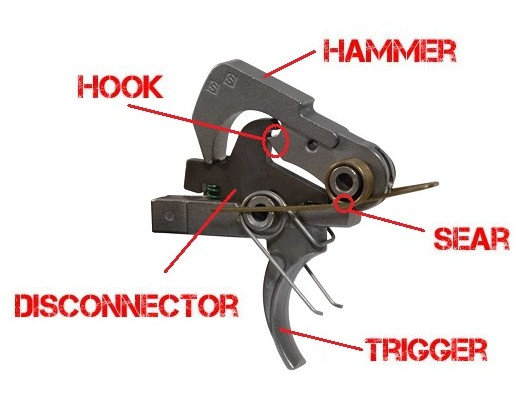
\includegraphics[width=0.5\textwidth]{../Figures/diagram-ar-15-trigger-assembly.jpg}
    \caption{AR-15 Firing Control Group \cite{AR15trigger} }
    \label{Firing Control Group}
\end{figure}



Our proposed solution is to block the firing control group by applying an additional force against the hammer, ensuring that it can never strike the firing pin. Our idea is to use a linear actuator to provide this force against the hammer. A linear actuator paired with a microcontroller would allow for low-voltage operation of our access control. The gun would then only be able to fire when a validated RFID tag is present in close proximity to our implemented system on the firing control group.

The primary contribution of this project is the integration of RFID-based access control into this already operating, small mechanical system. A passive RFID reader embedded near the control group continuously scans for a valid tag worn by the user, particularly in a ring worn on their finger. When an authorized tag is detected, the system signals the actuator to disengage, allowing normal operation of the firing mechanism. If no valid tag is present, the actuator blocks the hammer from hitting the firing pin. This way the firearm would never fire even if the trigger is pressed. This approach enables fast and implicit authentication without requiring user interaction, while also remaining low-power and cost-effective compared to biometrics alternatives. By combining a simple mechanical intervention with proximity-based RFID authentication, the system provides a practical solution for enhancing firearm safety. 